\setlength{\parindent}{2ex}
\begin{chapter}{Images and Blur}\label{chapter:introduction}
  \section{Introduction}
  In addition to being a rich source of artistic and creative value, images (or more precisely, visual data from projections of light) are an important source of scientific information.
  Even the word `observation' generally connotes visual perception, and its use as a catch-all for the measured verification of a hypothesis exemplifies the central role of vision in science.
  Many important scientific results have used visual data to discover and explain natural phenomena; for example, visual observations such as the color and shape of various plant organs in Gregor Mendel's experiments on hybridized peas formed the primary source of data for developing his model for genetic inheritance \citep{magner2002}.
  Arthur Eddington's 1919 image of the gravitationally lensed path of a comet during a solar eclipse provided the first experimental evidence supporting Albert Einstein's general theory of relativity \citep{eddington1920}.
%  The richness of the raw data content in an image and our human propensity to digest visual information -- the focus of our mind's eye, so to say -- make visual data in images a compelling source of scientific evidence and information.
  In these cases, only the \emph{qualitative} components of the visual response and their relationship to the experiment were relevant.
  With the advent of the camera, photosensitive chemistry, and later digital imaging technology, high-fidelity recording of visual observations as data became possible, allowing the potential to \emph{quantitatively} analyze visual information.
  Digital images when viewed quantitatively, can be described as the response of the incidence of light, and the subsequent exchange of energy, on a grid of regularly spaced grid elements, which we refer to as pixels.
  The ever-progressing technology in optical science and engineering are rapidly increasing the amount of data that can be measured in an image.
  Images are quickly becoming a source of `big data' in which new methods are rapidly being developed to extract information from this rich data source.
  Yet, there is a dichotomy between the amount of information available in image data and the complexity of how to quantitatively analyze it.
That is, despite having a large volume of data to extract information, their spatial nature makes measurements at each pixel highly dependent on measurements of adjacent pixels, and an objective extraction of information taking this structure into account is not obvious.
  A quantitative analysis of the image cannot assume that measured values are independent, because it is precisely this lack of independence that makes an image interesting -- independent image data is white noise (perhaps more appropriately, `gray noise') -- from which one can only infer the average of the measured pixels.

  In addition to the difficulties related to spatial dependence and high resolution, the structure of the data may have more components than spatial aspects since light is measured on a spectrum.
  That is, the energy response of light is not univariate since it is frequency dependent, and in many cases, is measured at several fixed bands of frequency.
  For example, astronomical images captured by the interstellar robotic probes Voyagers I and II measured 5 bands in the visible spectrum on a pixel grid with dimension $800 \times 800$ \citep{voyager}.
  In medical imaging, computed tomography (CT) is an imaging process where a series of axial measurements of attenuated electromagnetic radiation are used to reconstruct a cross-section of a scanned object, and the geometry of the measurement system is a primary source of complexity for quantitative analysis since data are organized in a non-Cartesian parameterization \citep{epstein2008}.
  The primary focus of this work is analyzing pulsed X-ray measurements, referred to as a radiographs, which are used as an experimental diagnostic of high-energy physics experiments.  
  Ultimately, analysis of the image is used to inform physical properties of the scene of interest, yet this measurement is indirect in several ways. 
  For example, in several high-energy radiographic imaging systems, collimated X-rays are pulsed through an experiment, then, the attenuated X-rays excite a crystal that responds by luminescing visible light at an intensity related to the energy of the attenuated wave-front.  
  The light is then focused and measured on a high resolution array (on the order of $1000\times1000$ or more) of charge coupled devices (CCD) calibrated to count photons at a specified spectral band.
  Each of these examples highlights the potential depth and complexity of modeling image capture, and models must be sufficiently flexible in order to be realistic and reliable.
  Our approach will be to remove the constraints of a parametric form for describing the process of image blur so that we have more flexibility in capturing the effects of aggregate complexity, as well as allowing data to better characterize the form of the model. 

A classical approach to quantitative image analysis is via a field of applied mathematics known as signals processing.
A general treatment is to model image capture as the response to a system where an ideal image or signal is filtered by some process forward modeled by the physics of the system and stochastic measurement effects. %, then the filtered observed data is observed.
The ideal image is then estimated indirectly by `reversing' the forward filter. 
When this process is modeled as an operator between function spaces, tools from functional analysis can be used to `solve' the system.
See one of the books \citep{vogel2002,epstein2008} for an in depth discussion and broad set of examples.

Relatively recently, techniques and ideas from formal data science have been used to not only model the measurement as stochastic, but also the unknown ideal image. 
Bayesian techniques provide a natural way to incorporate prior knowledge as well as uncertainty in that knowledge.
Formally, an image is modeled as a random field, and its correlation structure is the primary focus of study.
Under the assumptions of a Gaussian Markov random field, the correlation and mean completely describe the stochastic properties of the image \citep{rue2005gaussian}.
The books \citep{cressie1993statistics,rue2005gaussian} provide an excellent overview of the history and current methods for statistical methods for spatial data.
The field of spatial statistics, and more broadly random fields,  has had much development over the past half-century and has inspired a wealth of theory and computational tools, but is far from complete.
Moreover, more than applied mathematicians and statisticians have studied images quantitatively.
  A broad field of scientific disciplines has considered image-like data in one way or another; fields such as astronomy, astrophysics, biology, medicine, geology, computer science, and nuclear physics to name a few.
Each have a unique perspective on the problem, and a vast literature on the subject has accumulated.
Although much work has been done, it is still a very active research area and is far from the level of consensus and understanding that analysis of independently sampled data has achieved. 
The aim of this work is to develop and adapt current models and methods for estimation and quantifying uncertainty to the specific component of image analysis related to blur introduced by the system for capturing images.
Understanding this is an important component to the development and analysis of methods for quantitatively analyzing the images themselves.

\subsection{Organization}
This dissertation consists of four, more or less, independent chapters that address novel contributions to aspects of modelling and estimating the point spread function for an imaging system that exhibits translation invariant and radially symmetric blur.

The remaining sections of this chapter provide the general background for modeling image blur, and introduces how blurred images can be modeled with integral convolution with a point spread function (PSF).
We develop a flexible non-parametric model for image blur that allows for estimation of the .
The main goal of this work will be to estimate this quantity in a rigorous way that also incorporates uncertainties of the estimate.
The model we develop is completely novel, and the development is substantially more general than other parametrically dependent methods currently used.
The modeling perspective will provide several mathematical forms (e.g.~by changing variables) for describing the blurring of an opaque edge, with each providing a different insight into the process.
 We emphasize that each of these forms do not change the physical assumptions of the model, and are used to prove and understand various aspects of the underlying, intrinsic operation. 
Moreover, each of these different mathematical formulations provide several methods for analysis, e.g.~one formulation shows that a blurred edge is sufficient for estimation, and another is useful for seeing that the problem is ill-posed.  
In this process, we will also show connections with other operator based models of active interest; specifically, the Radon and Abel transform.

  In the next chapter, we will derive the necessary theory and technical definitions to formally define the operator between separable Hilbert spaces.
  Again, this development will take several perspectives, but not change the fundamental action.
  The analysis provides a fundamental notion of the interaction of radially symmetric objects with non-radially symmetric objects.
  \Cref{chapter:theoretical} will be mainly theoretical, but the explicit forms for the discrete model of the forward operator and prior information are motivated and derived there.
  This chapter will use tools from the theory of distributions for partial differential equations (PDEs) to develop a novel notion of symmetry that retains the powerful structure of a complete inner product space. 

  For estimation, we take a Bayesian approach which will allow for uncertainty quantification of the estimate, and \Cref{chapter:mcmctheory} will lay out prerequisite Markov Chain theory and the general algorithms based on it that are used in this work.
  We derive and describe from first principles a recently developed enhancement to Gibbs sampling, that has has been independently derived and studied in several other works \citep{van2008partially,agapiou2014analysis}.
  Although stated without proof in \citep{van2008partially}, we provide a novel argument from first principles to prove an essential condition that has been overlooked in the literature for the invariance and ergodicity of the algorithm.
%  This chapter provides a novel argument that verifies an important property for the application of a newly developed enhancements to the Gibbs sampler.
  The algorithms presented in this chapter can be generally applied to statistical inference problems where simulating samples from a complicated density are required, and are not specific to PSF reconstruction.

  \Cref{chapter:computational} further develops these notions in order to carry out PSF estimation on a computer, and gives detailed descriptions of the algorithms and associated probability densities so that they can easily be adapted for a standard scientific or statistical software suite. 
  We will also deal with how to discretely represent each of the necessary components in the estimation problem.
  Finally we present results from an implementation of the methods using the \textsc{Matlab} computing software library on synthetically derived and measured radiographic data.
  The measured data are from a high-energy X-ray imaging system at the U.S.~Department of Energy's Nevada National Security Site.
  We will end with a discussion of conclusions and possible future work.

\section{Modeling blur with a PSF}
  
  One major component of the spatial relationship of neighboring pixels of an image is due to blur from the imaging instrumentation.
  That is, under the assumption that arbitrary images are consistently measured by the modeled system, what contribution does this system have on how pixels are related, and how can we quantify this relationship?
  A widely used model for blurring \citep{hansen2010,jain1989,vogel2002,epstein2008} expresses this relationship as a linear filter that maps an ideal image $f$ to a blurred image $b$ by integrating
  %this relationship through a point-wise integral product with a function that describes interaction with neighboring points, e.g.
\begin{equation}\label{eq:generalFilterForm}
  b(x,y) = \iint_{\R^2} k(x,y;s,t) f(s,t)\,dsdt,
\end{equation}
  where $b(x,y)$ represents the intensity of the blurred image at $(x,y)$; $f(s,t)$ represents the intensity of the ideal un-blurred image at $(s,t)$; and $k$ is the kernel of the filter, which characterizes the blurring process.
  For the purpose of modeling, we assume that each function is sufficiently regular so that each integral and change of variable can be interpreted in the Riemann sense.

  Informally, the effect of blur can be viewed point-wise by observing the system response of a `point-source' at $(\bar x,\bar y)$, %(formally, take $f = \delta_{\bar x,\bar y}$, Dirac's delta translated to $(\bar x,\bar y)$) 
  then $b(x,y) = k(x,y;\bar x,\bar y)$ represents the ``spread'' at the point source.
  The function $k$ is referred to as the \emph{point spread function} (PSF) of the system at $(\bar x,\bar y)$.
  When the effect of blurring does not depend on the location of this point, that is, translating the ideal image $f$ by $(\bar x, \bar y)$ results in the blurred image $b$ also being translated by $(\bar x,\bar y)$, we say that the blur is \emph{spatially invariant}. 
  This means
\begin{align} 
  b(x-\bar x,y-\bar y) 
  &= \iint_{\R^2} k(x,y;s,t) f(s-\bar x,t - \bar y)dsdt \nonumber\\
  &= \iint_{\R^2} k(x,y;s'+\bar x,t'+\bar y) f(s',t')ds'dt'.\label{eq:convDerive1}
\end{align}
  On the other hand, applying the translation to \eqref{eq:generalFilterForm} implies
\begin{equation} \label{eq:convDerive2}
  b(x-\bar x,y-\bar y) = \iint_{\R^2} k(x-\bar x,y-\bar y,s,t) f(s,t)dsdt. 
\end{equation}
  Since \eqref{eq:convDerive1} and \eqref{eq:convDerive2} hold for all $f$, we have for each $x,y,\bar x, \bar y,s,$ and $t$ that
\begin{align} 
 k(x,y;s+\bar x,t+\bar y) = k(x-\bar x;y-\bar y,s,t) 
\end{align}
  and, in particular, when we fix $(s,t) = (0,0)$,
\begin{align} 
 k(x,y;\bar x,\bar y) = k(x-\bar x,y-\bar y;0,0).
\end{align}
Hence, the PSF in the blurring operation is independent of translation by $(\bar x,\bar y)$.
  Let us denote $k(x,y;\bar x,\bar y) = k(x-\bar x,y-\bar y)$, then the linear filter in \eqref{eq:generalFilterForm} reduces to   
\begin{equation}\label{eq:deconvolutionProblem}
  b(x,y) = \iint_{\R^2} k(x-s,y-t) f(s,t)\,dsdt.
\end{equation}
  Equation \eqref{eq:deconvolutionProblem} is called the \emph{convolution} of $f$ by $k$.
  In fact, any translation invariant linear filter described as an operator between $L^p$ spaces can be expressed through convolution with some generalized function $k$ \citep{grafakos2014}.
  In any case, when blur is assumed to be spatially invariant, it results in solving the convolution equation \eqref{eq:deconvolutionProblem}.
  Mathematical methods that estimate $f$ given $b$ and $k$ are referred to as \emph{deconvolution} techniques.

  Note that a change of variables by $s'=x-s$ and $t'=y-t$ results in a convolution of $k$ by $f$, which is to say that convolution, as an operation, is symmetric.
  That is
\begin{equation}\label{eq:dualConvolutionDeterministic}
  b(x,y) = \iint_{\R^2} k(s,t) f(x-s,y-t)\,dsdt.
\end{equation}
  This dual relationship between the PSF and the image will allow us to use the framework and many of the tools of deconvolution for the problem of PSF estimation.
  That is, we will use a known ideal $f$ to estimate the PSF $k$.

  Typically, deconvolution methods assume that the form of the PSF can be accurately described by modeling the imaging system \citep{jain1989,hansen2010}, but for X-ray radiography this is not realistic.
  If instead the imaging system is designed so that repeated images can be taken under consistent conditions, then by convolution symmetry in \eqref{eq:dualConvolutionDeterministic}, the blurring of a known calibration image can be cast as deconvolving the PSF from the ideal $f$ corresponding to the known image.

  Recall that the PSF models the blurring response of a single point, so a direct estimate of $k$ can be obtained by imaging a bright point-source, which approximates the impulse response to \eqref{eq:dualConvolutionDeterministic}.
  In astronomical imaging, the point-source can be a bright distant star, or in a controlled setting where visible light is measured, a focused laser provides a good point-source estimate \citep{tomaney1996expanding}.
  However, in the spectral regime of X-rays, focusing the high-frequency light is notoriously difficult and usually is impractical in situations of interest, so a point-source estimate of the PSF is usually unavailable. % at these frequencies.
  Instead, the system response of a uniformly opaque calibration object with a simple geometry can be measured.
  Under the assumption that the object is sufficiently thick so that X-rays are completely attenuated on the profile of the object, the function for the ideal image is given by an indicator function on a set $E \subseteq \R^2$ determined by the object's profile.
  Calibration objects typically have simple geometry and reduce the complexity of solving the deconvolution problem in \eqref{eq:dualConvolutionDeterministic}.  
  For example, the object could be a circular aperture or two perpendicular edges aligned with the imaging plane \citep{doering1992,watson1993}.
  As will be seen, the additional assumption of radial symmetry on $k$ is sufficient to estimate the PSF from the calibration image of straight edge. 
  Specifically, if the calibration object completely attenuates X-rays along a vertical edge at the fixed location at $s=0$ in the imaging plane, then $E=\{(s,t):s\ge0\}$ and $f_E(s) \eqdef f(s,t) = 1$ if $s\ge0$ and $0$ if $s <0$; see \Cref{fig:edgePicture} for a schematic of the calibration object in the measurement system and \Cref{fig:edgeData} for an example of recorded intensity data.
  The model for blur in \eqref{eq:dualConvolutionDeterministic} reduces to
\begin{equation}\label{eq:psfForwardModelDeterministic2D}
  b(x,y) = \iint_{\R^2} k(s,t) f_E(x-s)dsdt. 
\end{equation}
  Note that $b$ does not depend on $y$ in \eqref{eq:psfForwardModelDeterministic2D}, so denoting $b(x) = b(x,0)$, \eqref{eq:psfForwardModelDeterministic2D} reduces to
\begin{equation}\label{eq:psfForwardModelDeterministic}
  b(x) = \iint_{\R^2} k(s,t) f_E(x-s)dsdt. 
\end{equation} 
  
  In general, estimating $k$ from $b$ in \eqref{eq:psfForwardModelDeterministic} is underdetermined, since there are many distinct $k$ that can result in the same output $b$.
  To see this, note that 
  \begin{equation}
    \int_{-\infty}^{\infty} te^{-t^2 - s^2}dt = 0
  \end{equation}
  for all $s$ since the integrand is odd in $t$, and given any solution $k$, $k(s,t)+te^{-t^2 - s^2}$ also satisfies \eqref{eq:psfForwardModelDeterministic}.
  Observe that these PSFs are not radially symmetric.
  It will be seen in the next section that the assumption of radial symmetry on $k$ is sufficient for a unique solution to \eqref{eq:psfForwardModelDeterministic}.
%In summary, we've assumed that the effect of blur is modelled by a spatially invariant linear filter with a radially symmetric kernel, and \eqref{eq:psfForwardModelDeterministic} describes the blurring of a calibration object whose profile is an edge.
  Solving the integral equation in \eqref{eq:psfForwardModelDeterministic} is the primary focus of this work.
%The form of \eqref{eq:psfForwardModelDeterministic} is not immediately useful for analyzing the problem, and in the next sections, we will transform variables in \eqref{eq:psfForwardModelDeterministic} in two different ways that will show that the PSF estimation problem fits within the broad category of mathematical study known as \emph{inverse problems}.

\begin{figure}
  \begin{center}
    \begin{tikzpicture}[scale=.8,every node/.style={minimum size=1cm},on grid]
      \def\myxslant{0.1}
      \def\myyslant{-0.4}

	\begin{scope}[
		xshift=40,
		every node/.append style={
		xslant=\myxslant,yslant=\myyslant},xslant=\myxslant,yslant=\myyslant
	]
	\draw (0,0) rectangle (2.8,2.2);
%	\draw[fill=black] (1,0) rectangle (2.8,2.2);
	\end{scope}

	\begin{scope}[
		yshift=-20,
		every node/.append style={xslant=\myxslant,yslant=\myyslant},
		xslant=\myxslant,yslant=\myyslant
	]
	\draw[x=.314cm,y=.2cm,z=.2cm,thick,-latex,red] (0,0,0)
	  sin ++(0,1,1) cos ++(0,-1,1) sin ++(0,-1,1) cos ++(0,1,1)
	  sin ++(0,1,1) cos ++(0,-1,1) sin ++(0,-1,1) cos ++(0,1,1)
	  sin ++(0,1,1) cos ++(0,-1,1) sin ++(0,-1,1) cos ++(0,1,1);
	\draw[x=.314cm,y=.2cm,z=.2cm,thick,-latex,red] (-2,0,0)
	  sin ++(0,1,1) cos ++(0,-1,1) sin ++(0,-1,1) cos ++(0,1,1)
	  sin ++(0,1,1) cos ++(0,-1,1) sin ++(0,-1,1) cos ++(0,1,1)
	  sin ++(0,1,1) cos ++(0,-1,1) sin ++(0,-1,1) cos ++(0,1,1);
	\draw[x=.314cm,y=.2cm,z=.2cm,thick,-latex,red] (-4,0,0)
	  sin ++(0,1,1) cos ++(0,-1,1) sin ++(0,-1,1) cos ++(0,1,1)
	  sin ++(0,1,1) cos ++(0,-1,1) sin ++(0,-1,1) cos ++(0,1,1)
	  sin ++(0,1,1) cos ++(0,-1,1) sin ++(0,-1,1) cos ++(0,1,1);

	\pgfmathsetmacro{\cubex}{2}
	\pgfmathsetmacro{\cubey}{2.5}
	\pgfmathsetmacro{\cubez}{1}
	\draw[black,fill=gray,opacity=.75] (3.7,3,0) -- ++(-\cubex,0,0) -- ++(0,-\cubey,0) -- ++(\cubex,0,0) -- cycle;
	\draw[black,fill=gray,opacity=.75] (3.7,3,0) -- ++(0,0,-\cubez) -- ++(0,-\cubey,0) -- ++(0,0,\cubez) -- cycle;
	\draw[black,fill=gray,opacity=.75] (3.7,3,0) -- ++(-\cubex,0,0) -- ++(0,0,-\cubez) -- ++(\cubex,0,0) -- cycle;

	\draw[x=.314cm,y=.2cm,z=.2cm,thick,-latex,red] (4,0,0)
	  sin ++(0,1,1) cos ++(0,-1,1) sin ++(0,-1,1) cos ++(0,1,1)
	  sin ++(0,1,1) cos ++(0,-1,1) sin ++(0,-1,1) cos ++(0,1,1);
	\draw[x=.314cm,y=.2cm,z=.2cm,thick,-latex,red] (2,0,0)
	  sin ++(0,1,1) cos ++(0,-1,1) sin ++(0,-1,1) cos ++(0,1,1)
	  sin ++(0,1,1) cos ++(0,-1,1) sin ++(0,-1,1) cos ++(0,1,1);
	\end{scope}

	\begin{scope}[
		xshift=180,
		every node/.append style={xslant=\myxslant,yslant=\myyslant},
		xslant=\myxslant,yslant=\myyslant
	]
	    \draw (0,0) rectangle (2.8,2.2);
	    \tikzfading[name=fade left,left color = transparent!100,right color = transparent!0]
	    \draw[path fading=fade left,fading transform={rotate=-30},fill=black] (.9,0) rectangle (1,2.2);
	    \draw[fill=black] (1,0) rectangle (2.8,2.2);
	\end{scope}

	\begin{scope}[
		xshift=300,
		every node/.append style={xslant=\myxslant,yslant=\myyslant},
		xslant=\myxslant,yslant=\myyslant
		]
	    \draw (0,0) rectangle (2.8,2.2);
	    \tikzfading[name=fade left,left color = transparent!100,right color = transparent!0]
	    \draw[path fading=fade left,fading transform={rotate=-30},fill=black] (.9,0) rectangle (1,2.2);
	    \draw[fill=black] (1,0) rectangle (2.8,2.2);
	    \draw[step=1mm, black] (0,0) grid (2.8,2.2); %defining grids
	\end{scope}
	

    %    %putting arrows and labels:
	\node at (2,2.5) (label1) {Opaque Edge};
	\draw[-latex,thick] (2,-2) to node[below] {Image System Response} (7.5,-2);
	\node at (4.65,-3.4) (math1) {$\displaystyle{b(x)=\iint_{\R^2} k(s,t) f(x-s)\,dsdt}$};

	\node at (7,2.5) (label3) {Blurred Profile};

	\node at (12,2.5) (label2) {Recorded Data};
	\draw[-latex,thick] (9,-2) to node[below]{Measurement error} (13.2,-2);
	\node at (11,-3.4) (math1) {$+\eps_x \sim N(0, \sigma^2)$};

    \end{tikzpicture}
  \caption{ A schematic of the measurement model for an X-ray image of an edge. An opaque block aligned with the imaging plane blocks light on the half plane to produce a blurred edge.}\label{fig:edgePicture}
\end{center}
\end{figure}

\begin{figure}
\begin{center}
  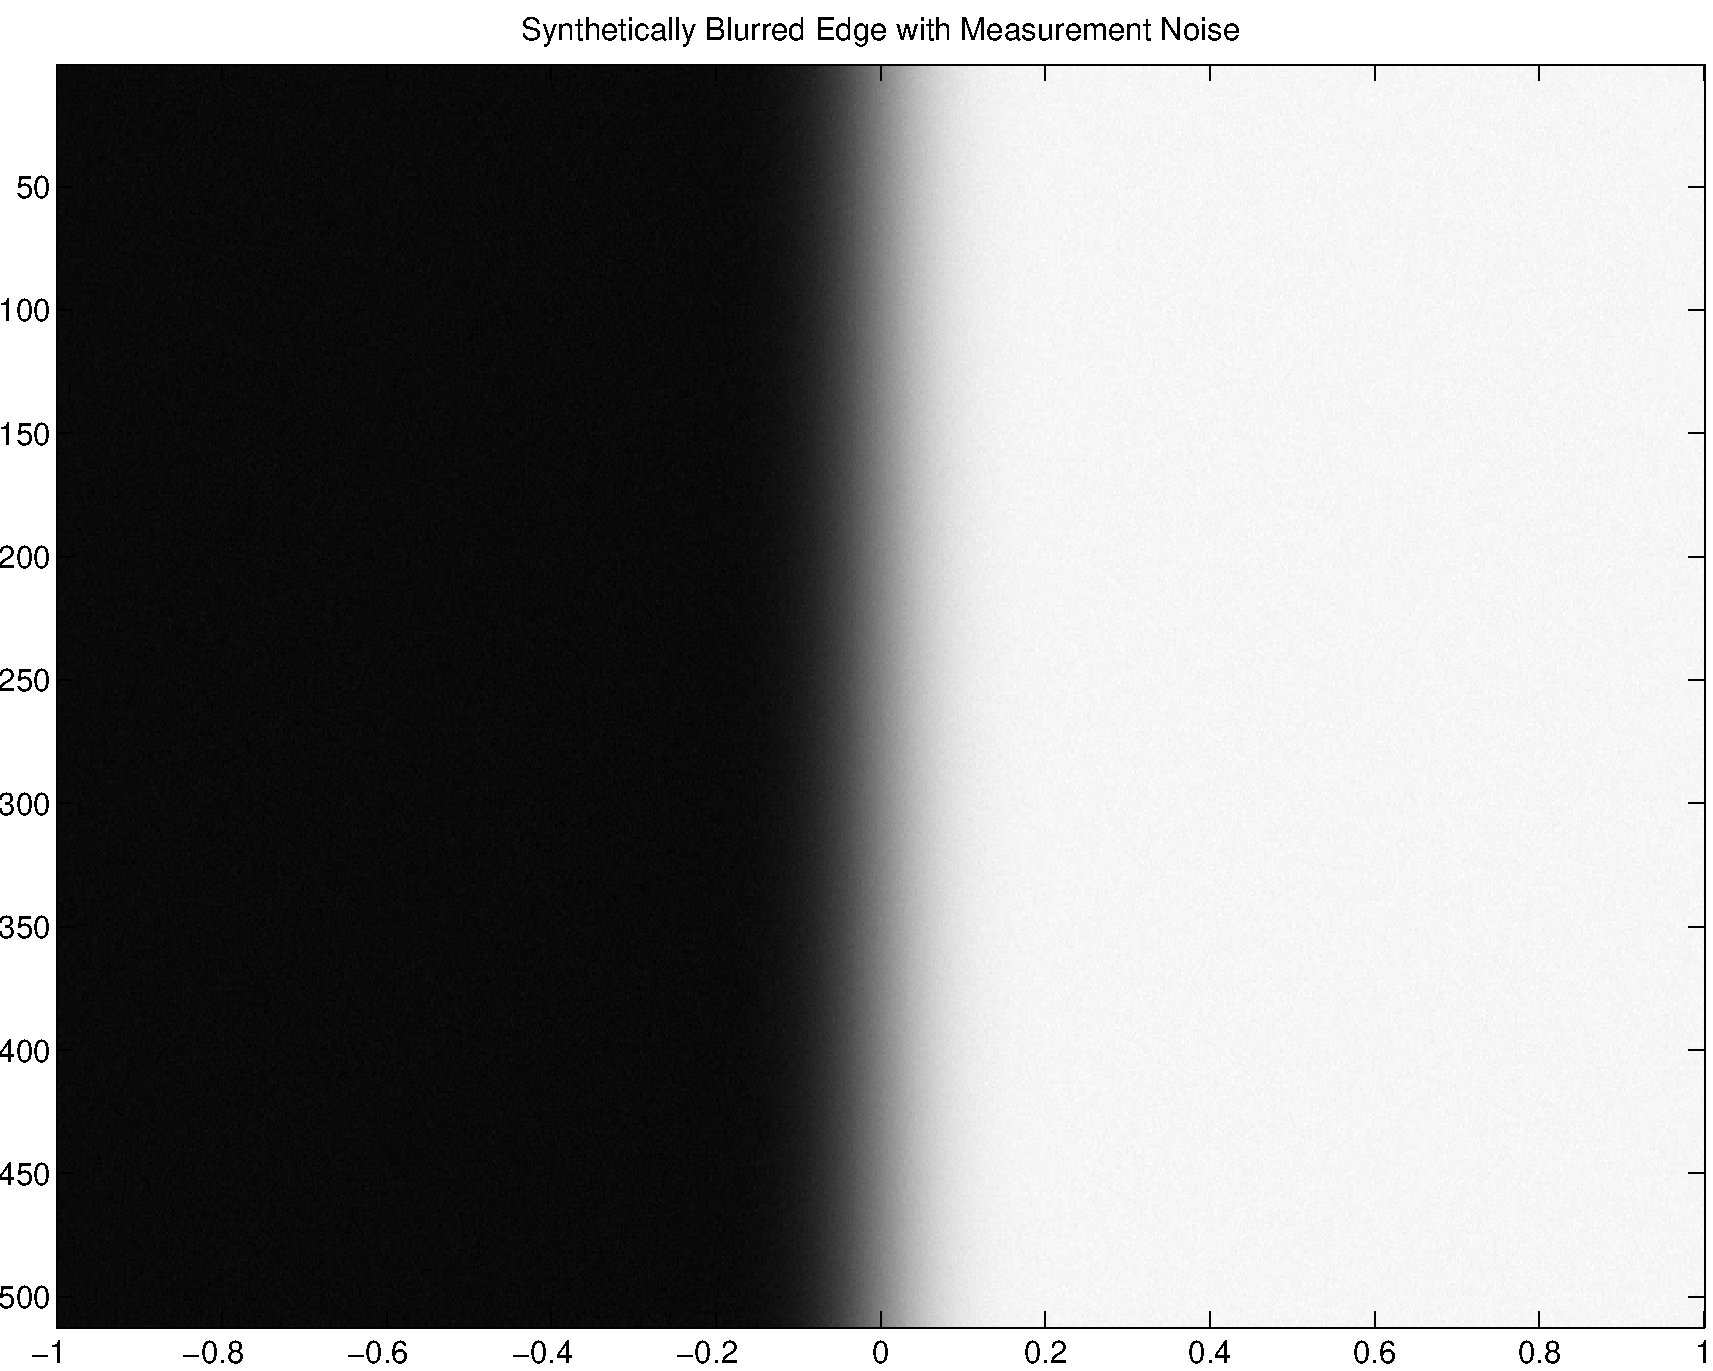
\includegraphics[width=.45\textwidth]{figures/blurredEdgeData.pdf}
  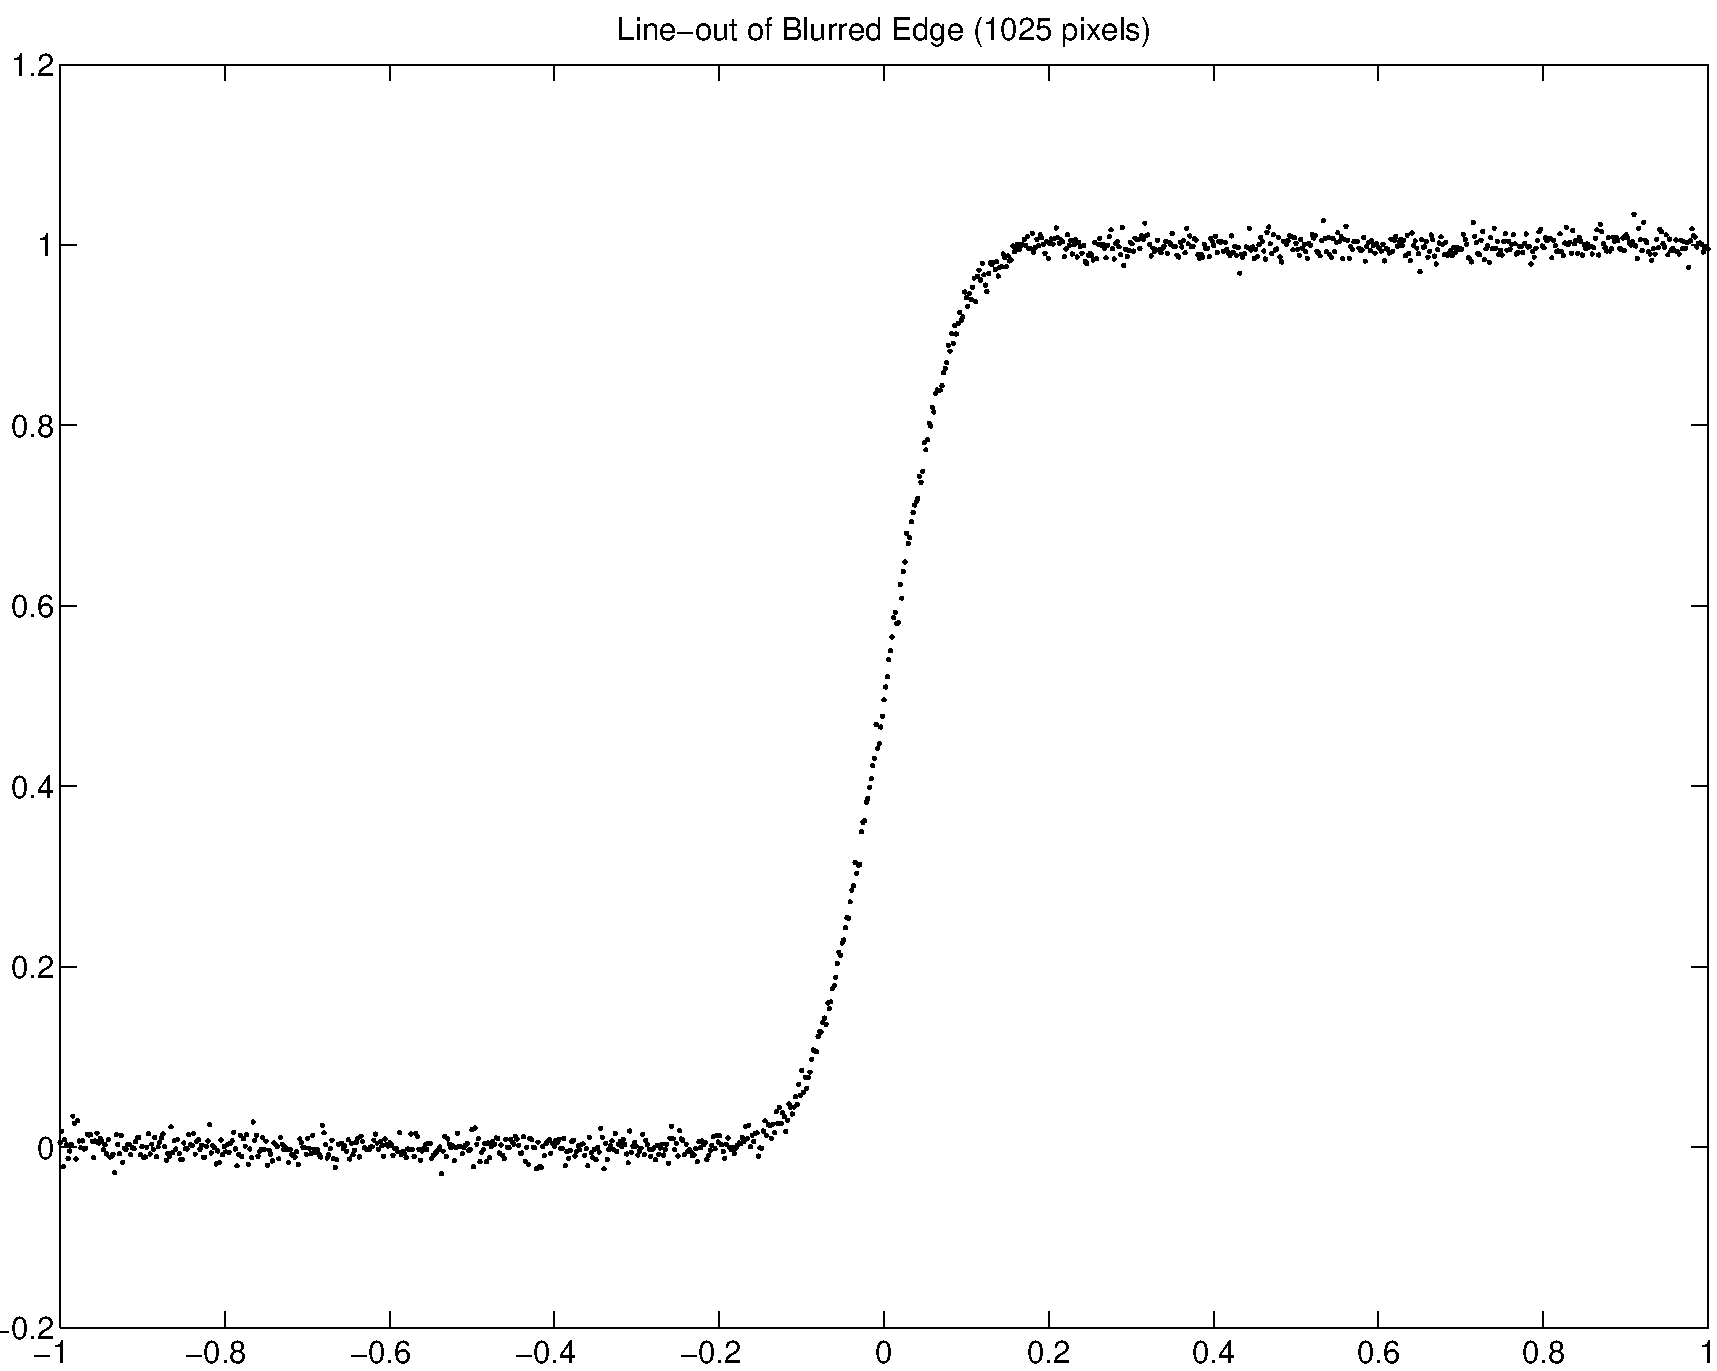
\includegraphics[width=.45\textwidth]{figures/psfLineoutData.pdf}
  \caption{A synthetically blurred edge with simulated measurement error and a line-out (horizontal cross-section) from the data.} \label{fig:edgeData}
\end{center}
\end{figure}
  
\section{The Abel transform and a deterministic solution}

  This section is devoted to explicitly deriving a solution to \eqref{eq:psfForwardModelDeterministic} and showing that radial symmetry is sufficient to guarantee a unique solution.
  This deterministic method offers useful insight into the problem, but will prove to be inadequate for practically obtaining estimates when the data is subject to measurement error.
%  This will lay out an solution to \eqref{eq:psfForwardModelDeterministic}. 
%  However, the suggested method will be problematic as will be seen in the following section.

%  A large part of designing a system for imaging is to minimize the effect of blur.
  Often, limitations due to physical laws put a lower bound on the measurement precision so that even an optimal design cannot ignore the effect of blur.
  Although arbitrary resolution may be impossible, it is often of interest to design a system that does not introduce error that is biased.
  A system that is not biased with respect to spatial orientation is said to exhibit \emph{isotropic blur}, so that, in the convolution model, the PSF is radially symmetric.
  In fact, many parametrically modeled PSFs assume radially symmetry \citep{doering1992,jain1989,kundur1996blind,watson1993}.  

  When one assumes that the PSF of their system is a radially symmetric continuous function on $\R^2$, then it has a unique representation on $\R$; i.e., for $k:\R^2 \to \R$, there exists a function $p:[0,\infty)\to \R$ so that $k(s,t) = p\left(\sqrt{s^2 + t^2}\right)$.  
  The function $p$ is referred to as the radial profile of $k$.
  Define
  \begin{equation} \label{eq:abelTransform}
    \ell(s) \eqdef \int_{-\infty}^\infty p\left(\sqrt{s^2 + t^2}\right)\,dt,
  \end{equation}
  which is integration along a line perpendicular to the edge $E$, and its form is commonly encountered in other imaging applications with radial geometry, such as tomographic imaging science.
  The transformation that takes $p$ to $\ell$ is known as the \emph{Abel transform}, and for its study in imaging science, see \citep{bracewell,epstein2008,knill93}.

  Viewing \eqref{eq:psfForwardModelDeterministic} as iterated integration first in $t$ allows $f_E(s-x)$ to be factored out of the inner integral. 
  Then substituting \eqref{eq:abelTransform} for $k$ into  \eqref{eq:psfForwardModelDeterministic} and changing the bounds of integration in $s$ according to $f_E(x-s)$, results in
  \begin{align}
    b(x) &= \int_{-\infty}^\infty f_E(x-s) \left(\int_{-\infty}^\infty p\left(\sqrt{s^2 + t^2}\right)\,dt\right)ds \nonumber \\
         &= \int_{-\infty}^x \left(\int_{-\infty}^\infty p\left(\sqrt{s^2 + t^2}\right)\,dt\right)ds \nonumber \\
         &= \int_{-\infty}^x \ell(s)ds. \label{eq:abelForward}
  \end{align}

  The graph of $b$ exhibits reflection symmetry about $(0,b(0))$.
  That is, for any $x>0$, the point $(0,b(0))$ is the mid-point between the points $(x,b(x))$ and $(-x,b(-x))$. 
  To see this explicitly, let $\tilde b(x) \eqdef b(x) - b(0)$, then for $x>0$
  \begin{align}
    -\tilde b(x) &= -\left(b(x) - \int_{-\infty}^0 \ell(s)ds\right) \nonumber \\
      &= -\int_0^x \ell(s)ds \nonumber \\
      &= \int_0^{-x}\ell(s')ds'  \nonumber \\
      &= b(-x) - b(0) \nonumber\\
      &= \tilde b(-x).
  \end{align}
  Hence $\tilde b(x)$ is odd and has reflection symmetry about the origin, hence, $b(x)$ has reflection symmetry about $(0,b(0))$.
  This means that data defined on either $x\in(-\infty,0]$ or $x\in[0,\infty)$ is sufficient for estimating $p$, since the other half is determined by symmetry.
  This observation will be important in the next section.

%  The collection of line integrals parametrized by their angle of incidence is called the Radon transform of $k$, and when $k$ is radially symmetric, the transform is completely determined by a single projection.
%  The operator that takes the radial profile $p$ to $l$ is called the Abel transform and is encountered in tomographic imaging.
  The Abel transform has an explicit expression for its inverse \citep{epstein2008} given by
  \begin{equation} \label{eq:inverseAbel}
    p(r) = -\frac{1}{\pi r} \frac{d}{dr}\left(\int_r^\infty \frac{\ell(s) s ds}{ (s^2 - r^2)^{1/2} } \right).  
  \end{equation} 
  The following calculations verify \eqref{eq:inverseAbel}.

  \begin{prop}
    Suppose that $p(r)$ is such $\lim_{r\to\infty}rp(r) = 0$ and $\ell(s)$ in \eqref{eq:abelTransform} is point-wise defined and the integral in \eqref{eq:inverseAbel} is finite for each $r$, then equation \eqref{eq:inverseAbel} holds.
  \end{prop}
  \begin{proof}
  We can express the inner integral in \eqref{eq:abelForward} as
  \begin{equation}
    \ell(s) = 2\int_{|s|}^\infty \frac{p(t) t}{(t^2 - s^2)^{1/2}}\,dt \label{eq:abelForward2}
  \end{equation}
  by symmetry of the integrand (it is even) and a change of variable by $r = s^2 + t^2$.
  Now, interchanging the order of integration in \eqref{eq:inverseAbel} results in
  \begin{align} 
    \left(\int_r^\infty \frac{\ell(s) s ds}{ (s^2 - r^2)^{1/2} } \right)  
    &= \int_r^\infty\int_s^\infty \frac{2p(t) ts}{(s^2 - r^2)^{1/2}(t^2 - s^2)^{1/2}}\,dtds \nonumber\\
    &= \int_r^\infty p(t) t\int_r^t \frac{2s}{(s^2 - r^2)^{1/2}(t^2 - s^2)^{1/2}}\,dsdt. \label{eq:inverseAbelderive1}
  \end{align} 
  In the second step, we have interchanged variables and the integral's support can be expressed 
  \begin{equation} \label{eq:inverseAbleSupport}
    \{(t,s): r \le s, s\le t\} = \{(s,t): r\le s \le t, r\le t \}.
  \end{equation}
  Another change of variables by $s^2 = \tau t^2 + (1-\tau)r^2$ (note $s\ge0$) results in $2sds = (t^2 - r^2)d\tau$, 
  so that the inner integral in \eqref{eq:inverseAbelderive1} is
  \begin{equation}
    \int_r^t \frac{2s}{(s^2 - r^2)^{1/2}(t^2 - s^2)^{1/2}}\,ds
    = \int_0^1 \frac {1}{\tau^{1/2}(1-\tau)^{1/2}}\,d\tau = \pi, \label{eq:gammaIntegral}
  \end{equation}
  where the last equality is given by an integral identity involving the gamma function.
%  Note that the resulting integral is independent of both $r$ and $t$, and hence, is constant. To evaluate it, recall the Gamma function identity
%  \begin{equation} 
%    \frac{\Gamma(\alpha)\Gamma(\beta)}{\Gamma(\alpha + \beta)} = \int_0^1 \tau^{-\alpha}(1-\tau)^{\alpha -1}\,d\tau,
%  \end{equation}
%  from which the expression in \eqref{eq:gammaIntegral} reduces to $\Gamma(1/2)^2 = \pi$.
  Collecting these results and applying the fundamental theorem of calculus with the assumption that $\lim_{r\to\infty}rp(r) = 0$ to \eqref{eq:inverseAbelderive1} implies
  \begin{align}
    -\frac{\pi}{r} \frac{d}{dr} \left(\int_r^\infty \frac{\ell(s) s ds}{ (s^2 - r^2)^{1/2} } \right) 
      &= -\frac{\pi}{r} \frac{d}{dr} \int_r^\infty p(t) t \pi dt \nonumber\\
      &= \frac{1}{r} \left(p(r)r - \lim_{r'\to\infty}p(r')r'\right) \nonumber\\
      &= p(r),
  \end{align}
  which proves the identity in \eqref{eq:inverseAbel}.
\end{proof}
  
  With this result, $p$ can be recovered from $b$ in \eqref{eq:abelForward} as follows: given $b(x)$, the fundamental theorem of calculus gives $\ell(x) + \lim_{x'\to\-\infty}\ell(x')$ by differentiating $b(x)$.
  Since $\lim_{r\to\infty}tp(t) = 0$, symmetry and the change of variables in \eqref{eq:abelForward2} implies $\lim_{x'\to-\infty}\ell(x') = 0$. 
  Then, applying the inversion formula in \eqref{eq:inverseAbel} to $b'(x)$ gives the radial profile $p(r)$.
  That is,
  \begin{equation} \label{eq:analyticInversion}
    p(r) = -\frac{1}{\pi r} \frac{d}{dr}\left(\int_r^\infty \left(\frac{d}{ds} b(s)\right) \frac{ s ds}{ (s^2 - r^2)^{1/2} } \right).  
  \end{equation}
  Hence, the assumption of radial symmetry sufficiently constrains the problem to uniquely determine the PSF from an edge calibration object illustrated in \Cref{fig:edgeData}.

  In theory, we have outlined a solution to the problem, but there is one more component to the model that has not been addressed -- random effects due to measurement error -- for which a direct application of the outlined method on measured data will fail spectacularly, due to the estimation problem being ill-posed, which we address in the next section.

\section{PSF reconstruction as an ill-posed inverse problem}
  
  The solution given by \eqref{eq:analyticInversion} will not be sufficient when measurement errors are introduced. 
  One clue that indicates this insufficy is that it requires taking derivatives of measured data, which is known to be problematic \citep{hanke2001}.
  In this section, we will return to \eqref{eq:psfForwardModelDeterministic}, and perform a different variable transformation to explicitly illustrate the instability, and in doing so, will derive a form that is more suitable for analysis and numerical discretization.

  The measurements of the imaging system are generally not deterministic and are subject to measurement noise.
  Precisely modelling the stochastic effect of measurement error is system dependent and can be quite complicated.
  In X-ray radiography, uncertainty can enter into the system at the luminescing crystal response, at the counts of CCD array, or through the electrical transmission of the signal.
  In order to be broadly applicable, and appealing generally to various central-limit-theorem-like results in probability \citep{durrett2010probability}, we model the stochastic measurement effect in aggregate as an additive, independent Gaussian noise process with zero mean and unknown variance.  
  For now, this assumption can be viewed as a small perturbation from the model, but its form will be important for the inference techniques developed in subsequent chapters.
  %The complete description of the model from which the PSF will be estimated is
  %  \begin{equation}\label{eq:psfForwardModelStochastic} 
  %    b(x) = \iint_{\Omega} k(s,t) f(x-s)dsdt + \eps_x  
  %  \end{equation}
  %where each $\eps_x \sim N(0,\sigma^2)$ and independently (in $x$) for some unknown variance $\sigma^2$.  

  Estimating a quantity of interest, in our case $k$, from indirect and noisy measurements, $b$, with a model where an operator takes $k$ to $b$ (referred to as the \emph{forward operator}) is called an inverse problem.  
  The problem is called well-posed when the forward operator is invertible, and the inverse is continuous. %inversion is insensitive to small perturbations.
  These famous conditions were laid in the early 20th century by \citep{hadamard1902}, but a number of important applications have arisen (among those computational imaging) where these conditions are violated; enough to the extent that the term `inverse problems,' as it refers to the mathematical research area, is exclusively devoted to solving ill-posed problems.
  In particular, most cases of interest %are when the measurement model results in data \emph{not} in the range of the model operator and 
  exhibit a model where the inverse of the forward operator is discontinuous.

  Returning to \eqref{eq:psfForwardModelDeterministic}, a variable transformation
  %(again assuming $\Omega$ is full measure in $\R^2$)  
  by $(s,t) = T(r,v) = (r\cos v,r\sin v)$, has $|dT(r,v)| = r$ and 
  \begin{align}
    b(x) &= \int_0^\infty p(r) \left( \int_{-\pi}^\pi f_E(x - r\cos v)dv \right)\,r dr\nonumber \\
         &= \int_0^\infty p(r) g(x,r) r dr, \label{eq:radialForwardModelDeterministic}
  \end{align}
where
\begin{equation} \label{eq:radialForwardKernel}
  g(x,r) \eqdef \left\{\begin{array}{lr}
    0 & x < - r\\
    2(\pi - \acos(x/r)) & |x| \le r\\
    2\pi &  x> r
  \end{array}\right..  
\end{equation}
  To see that $g$ has this form, note that integrating $f_E(x-r\cos v)$ is the radian measure of the set $\{v\in(-\pi,\pi): r\cos v \le x\}$; see \Cref{fig:radialForwardKernel}.  

\begin{figure}
  \begin{center}
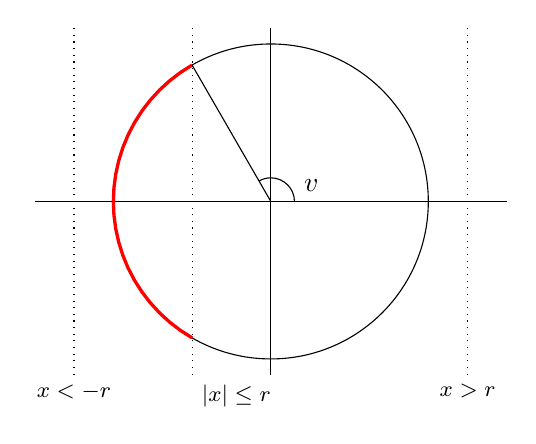
\begin{tikzpicture}
  \draw (0,-2.2) -- (0,2.2);
  \draw (-3,0) -- (3,0);
  \draw[dotted] (-2.5,-2.2) node[below]{\footnotesize$x<-r$} -- (-2.5,2.2);
  \draw[dotted] (2.5,-2.2) node[below]{\footnotesize$x>r$} -- (2.5,2.2);
  \draw[dotted] (-1,-2.2) node[below right]{\footnotesize$|x|\le r$} -- (-1,2.2);

  \draw (0,0) circle[radius=2];
  \draw[very thick,red,domain=120:240] plot ({2*cos(\x)},{2*sin(\x)});
  \draw (0,0) -- (-1,{sqrt(3)});
  \draw (.3,0) node[above right]{$v$} arc [radius=.3,start angle=0,end angle=120];
\end{tikzpicture}
  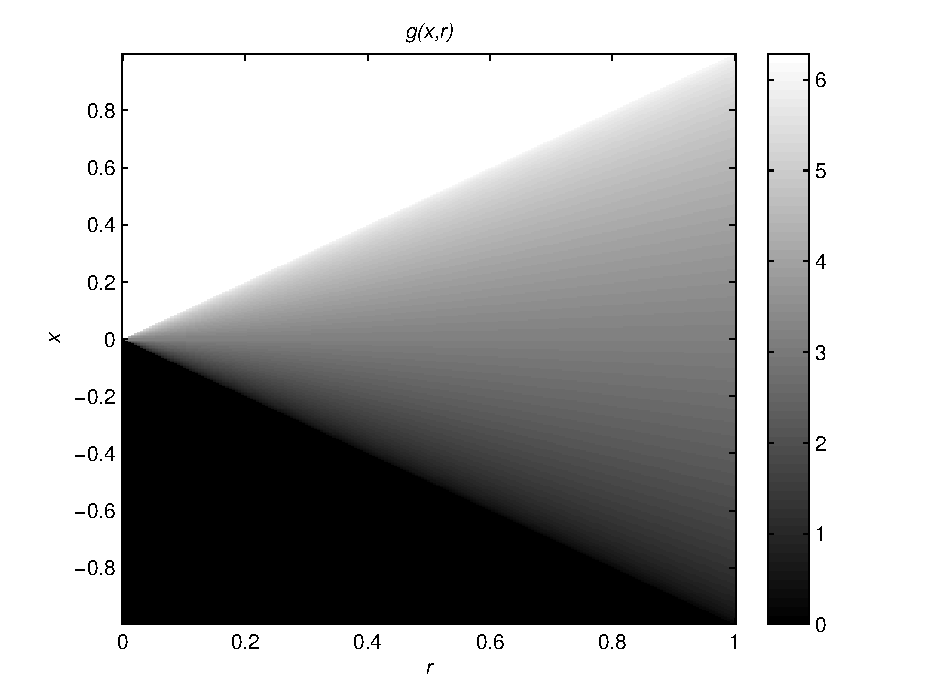
\includegraphics[width=.5\textwidth]{figures/g_function.pdf}
\end{center}
\caption{ The PSF forward integral operator kernel $g(x,r)$ represented as the arc measure of $v$ in $(-\pi,\pi)$ where $x \ge r\cos v$. }\label{fig:radialForwardKernel}
\end{figure}

  There are three key observations to make.
  From this viewpoint, the forward model is now a one-dimensional integral equation on the radial profile as opposed to the two-dimensional problem in \eqref{eq:psfForwardModelDeterministic}.
  Second, note that $g(x,r)$ is continuous (although it has a discontinuity in its partial derivatives across $r=s$).
  Finally, recall that the graph of $b(x)$ exhibits reflection symmetry about $(0,b(0))$.
  So, $b(x)$ defined on either $(-\infty,0]$ or $[0,\infty)$ completely determines $p$.

  The discussion thus far has been somewhat informal, as we have assumed that all functions are continuous and have not defined a space for the PSF, the domain of the forward operator denoted $\PP$, or the ambient space for the data, the codomain of the forward operator. %, so we have not formally defined the forward operator of the model.
  Defining these spaces rigorously is the main focus of \Cref{chapter:theoretical}, and it will be shown that both of these spaces are separable Hilbert spaces and, in particular, that the data are a subspace of $L^2((-\infty,0])$.
   For now, let $\G: \PP \to L^2((-\infty,0])$ be given and that the action of the operator is consistent with the integral equation in \eqref{eq:radialForwardModelDeterministic}, i.e., 
  \begin{equation}
    [\G p](x) = \int_0^\infty p(r) g(x,r) r dr.
  \end{equation}
  The operator $\G$ is a compact Hilbert-Schmidt operator since $g$ is continuous.
  Moreover, $\G$ is an injective operator since we showed that $b = \G p$ has an explicit solution. 
  The spectral theorem for such operators implies that $\G$ has a countable spectrum which has zero as a limit point, and hence, its inverse $\G^{-1}$ is unbounded. %, which results in an ill-posed problem. 
  See one of many texts on functional analysis such as \citep{bachman1966,rudin1991} for the spectral theorem regarding Hilbert-Schmidt operators, and \citep{tikhonov1963,vogel2002,morozov1993} for its role in inverse problems.
%  Each of these statements will be shown rigorously in \Cref{chapter:theoretical}.

  Solving ill-posed inverse problems requires prior assumptions about $p$ that regularize the unbounded inverse.
  Recall that the original formulation of the problem is cast in terms of deconvolution, and much of the literature of inverse problems is devoted to this subject. 
  This work draws heavily from techniques for that purpose, but has many nuanced differences that make the analysis challenging, yet also novel and interesting.
  We will utilize a Bayesian approach to analyzing the inverse problem, since in addition to estimating $k$, these techniques provide uncertainties in the resulting estimate and can be quantified by analyzing the so-called posterior distribution.
  These methods have been the subject of much recent research (see the books \citep{calvetti2007introduction,kaipo2005,stuart2010}), and the problem of PSF reconstruction fits neatly into that framework once the space $\PP$ and the forward operator have been well-defined, which we address in the next chapter.

\end{chapter}
